\documentclass[french,a4paper,12pt]{article} 
\usepackage[utf8]{inputenc}
\usepackage[T1]{fontenc}
\usepackage[a4paper,left=2cm,right=2cm,top=2cm,bottom=2cm]{geometry}
\usepackage{mathtools}
\usepackage[french]{babel}
\usepackage{libertine}
\usepackage{blindtext}
\usepackage{babel}
\usepackage[pdftex]{graphicx}
\usepackage{lmodern}
\usepackage{url}
\setlength{\parindent}{0cm}
\setlength{\parskip}{1ex plus 0.5ex minus 0.2ex}
\newcommand{\hsp}{\hspace{20pt}}
\newcommand{\HRule}{\rule{\linewidth}{0.5mm}}
\selectlanguage{french}
\title{BP} % le titre de l'article
\author{Marina Cathy Beaujolais} 
\usepackage{caption,subcaption}
\tracinglostchars=2
\usepackage{iftex}
\pagestyle{empty}
\usepackage[authoryear]{natbib}
\ifTUTeX
  \usepackage{fontspec}
\else
  \usepackage[T1]{fontenc}
  \usepackage[utf8]{inputenc} % The default since 2018
  \DeclareUnicodeCharacter{200B}{{\hskip 0pt}}
\fi
\usepackage[]{tocbibind}

\begin{document}
\begin{titlepage}
  \begin{sffamily}
  \begin{center}
    
    
\includegraphics[scale=0.25]{logoulb.JPG}~\\[1.5cm]

    \textsc{\bfseries \LARGE Université Libre de Bruxelles }\\[0.5cm]
    \textsc{\Large Faculté de Lettres, Traduction et Communication}\\[6cm]

    % Title
    \HRule \\[0.4cm]
    { \huge \bfseries Sujet n°6 :​Évaluer les services​ d’une bibliothèque publique\\[0.4cm] }

    \HRule \\[4cm]
    % Author and supervisor
    \begin{minipage}{0.4\textwidth}
      \begin{flushleft} \large
        Aubert Marina \\
        Metango Kenfack Cathy \\
        Yepmou Beaujolais \\
        
      \end{flushleft}
    \end{minipage}
    \begin{minipage}{0.4\textwidth}
      \begin{flushright} \large
        \emph{Travail réalisé sous la direction de M. Christian Brouwer dans le cadre du cours Gestion des Bibliothèques (M-STIC-B420)} 
      \end{flushright}
    \end{minipage} \\ [2cm]

    \vfill

    % Bottom of the page
    {\large {} Année académique 2022-2023}

  \end{center}
  \end{sffamily}
\end{titlepage}


 %%fin de la parge de garde 
 \begin{center}
 \tableofcontents
 \end{center}
\newpage



\section{INTRODUCTION}




\newpage
\section{METHODOLOGIES}
Pour chaque étape du travail,  
Notre première étape a été de reformuler et de cadrer le thème du travail de groupe. 

\quad Nos questions de départ ont ainsi été formulées ainsi : Quels sont les services d'une bibliothèque publique ? Comment sont-ils évalués par rapport à leurs différents publics ? Comment les résultats de ces évaluations impactent-elles l'évolution de ces services ?\\
 
\subsection{Méthode de recherche​ et Équations de recherches}
\quad Premièrement, nous avons décidé de concentrer la recherche sur les sources en français et en anglais, les langues que nous maîtrisons. Deuxièmement, nous limiterons notre recherche bibliographique sur des publications académiques revues par des pairs, les plus robustes scientifiquement parlant. Troisièmement, nous viserons principalement la période située entre 2000 et 2022 : cette période de temps correspond à l’émergence des nouvelles technologies, et à la nécessité pour les bibliothèques publiques de s’y adapter. Elle nous permet donc d’évaluer à la fois les services traditionnels, présents depuis le début de la période, mais aussi les services directement liés aux nouvelles technologies, et enfin les nouveaux services, indirectement provoqués par cette nouvelle manière d'envisager le rôle des bibliothèques publiques. 

A partir de la bibliographie fournie, nous avons réalisé une première sélection de sources. Celle-ci a permis à Cathy et Beaujolais de réunir douze titres de périodiques et quinze livres. 

Parallèlement, Marina a élaboré l’équation de recherche, en français et en anglais, afin de lancer des recherches dans les instruments de travail de la bibliographie fournie :\textbf{ ((évalu* OR appréci* OR estim* OR examin*) AND services AND "bibliothèque* publique*") OR ((evalu* OR appr* OR estimat* OR valu* OR assess*) AND services AND "public librar*") }

Des niveaux différents de difficulté ont été rencontrés lors de l’utilisation de cette équation de recherche. La recherche dans la base de données @SIC n’a pas posé de difficultés, elle a délivré septante résultats. La recherche dans LISTA a généré trop de bruit, et Marina a dû activer des filtres limitants, et supprimer la recherche à des sujets équivalents ; finalement, cent soixante-et-un résultats ont été reçus. La recherche dans IFLA a résulté en un trop grand silence : la recherche a été lancée uniquement anglais, sans synonymes ; six résultats ont été délivrés.  

Les trois membres du groupe se sont réparti la sélection des sources parmi ces cent seize résultats. Finalement, notre corpus final a réuni cent-quarante-trois sources.  \\

\subsubsection{ Outils de gestion bibliographique : Zotero}
\quad Nous avons encodé notre corpus dans Zotero en préparation de la bibliographie de notre travail. Les sources ont été encodées en leur associant le type de services à évaluer (services traditionnels, services liés aux nouvelles technologies, nouveaux services), et les méthodologies d'évaluation à envisager (évaluations quantitatives (statistiques, enquêtes d’usage, enquêtes de satisfaction, méthode de Kantor, enquêtes de qualité), évaluations qualitatives (entretiens individuels, méthodes ethnographiques, écoute du personnel), indicateurs de performance). Nous avons élaboré ces mots-clés sur base du cours de Gestion des bibliothèques. Nous avons écarté les normes ISO qui évaluent l'impact des bibliothèques publiques, et non leurs services. 

En encodant notre corpus, Zotero a intégré de nouveaux mots-clés pour qualifier nos sources. Afin d’obtenir une vue hélicoptère de l’ensemble des sources, nous avons décidé de réaliser un travail d’affinage des mots-clés avant d’entrer dans l’analyse de nos sources pour l’état de l’art. Nous avons donc décidé de d’abord supprimer les mots clés liés aux situations géographiques, aux auteurs, et les doublons, de conserver les mots-clés qui décrivent des services ou des modes d'évaluation, et d’ensuite préparer un plan détaillé de l’état de l’art, avant de procéder à la rédaction. 

C’est à ce stade que nous avons exposé notre démarche à la classe via une présentation Powerpoint ; ce dernier a été créé au fur-et-à-mesure de nos échanges sur la création de notre méthodologie et sur la répartition du travail. \\

\subsubsection{Référencement }
Nous nous sommes basés sur le cours elearning « What’s up doc » de l’Université virtuelle pour identifier le mode de référencement : (auteur, année)

\subsection{Répartition du travail entre les membres du groupe}
\quad Dès le début du projet, l’ensemble du travail a été divisé en quatre étapes : la constitution du corpus, la rédaction de l'analyse pour l’état de l’art, les études de cas, la finalisation. Pour chaque étape, le travail a été réparti de manière équitable entre les trois membres de l’équipe. \\

Chaque étape ou partie d’étape a été cadrée par une date d’échéance et des dates de rencontre, soit en bibliothèque, soit en visioconférence. \\

La rédaction est réalisée en latex avec Texmaker et Miktex, coordonnée via Github. Ce choix d’outil nous permet d’intégrer facilement le référencement de Zotero, et nous permet de nous entraîner pour la rédaction de nos prochaines rédactions pour le master. \\

\subsection{Planing d'exécution du Projet}





\newpage
\section{Etat de l'art}

\quad Lors du travail sur les mots-clés, Cathy s’est rendu compte que les sources avaient disparues de Zotero. Beaujolais et Marina ont réussi à récupérer les données perdues grâce à la sauvegarde automatique de Zotero. Ce sauvetage a pris plusieurs jours, a généré des sources en doublon à fusionner, et nous a imposé de réfléchir à une autre manière de réaliser l’Etat de l'art : nous avons renoncé à supprimer les mots-clés de Zotero, et estimé que nous allions chacune et chacun consulter les mots-clés en fonction de nos services à évaluer. 

Cathy se concentre sur l’évaluation des services traditionnels, Beaujolais sur l’évaluation des services liés aux nouvelles technologies, et Marina sur l’évaluation des nouveaux services.
\subsection{Methodes d'évaluation}

\subsubsection{Méthodes quantitatives}


\subsubsection{Méthodes qualitatives}


\subsection{Evaluation des services traditionnels}




\subsection{Évaluation des services liés aux nouvelles technologies}
\quad D'après LAROUSSE, le terme Nouvelles technologies signifie :\textit{ moyens matériels et organisations structurelles qui mettent en œuvre les découvertes et les applications scientifiques les plus récentes. (On dit aussi haute(s) technologie(s), technologie(s) de pointe, technologie(s) avancée(s).)}\\
 
 
 
 Toute au long de cette section, nous étudierons l’enjeu en mettant l’accent sur l’importance de la mise en place des normes et statistiques afin d'évaluer l’impact des services liés nouveaux technologies sur les bibliothèques publiques.\\
 
 
\subsubsection{Approches d'évaluation des services électroniques}
\quad La définition d'e-service ou Services électroniques dans le dictionnaire est l'utilisation de la technologie électronique par une organisation pour fournir des services à ses clients. 
 XXXXXXXXXXXXXXXXXXXXXXXXXXXXXXXXXXXXXXXXXXXXXXXXXXXXXXXXXXXXXXXXXXXXXXX\\[4cm]
 
 selon Peter R. <<\textit{Il se peut que la nouvelle offre de services électroniques entraîne, de manière fondamentale, la refonte de la statistique quantitative en bibliothèque}>>, refonte qui pourrait s’appuyer sur une évaluation construite sur la combinaison des approches suivantes\citep{young1998evaluation}:
\begin{enumerate}
\item[•]\textbf{Mesures fondées sur les transactions :} les sessions interactives, les téléchargements, le volume d’informations obtenues rapporté au nombre de terminaux et d’utilisateurs, les domaines et les adresses des serveurs, les images ou les fichiers sont comptés, enregistrés et mesurés par sondages ou par relevés de transaction.
\item[•]\textbf{Mesures fondées sur la durée de connexion :} les horaires de fonctionnement, la durée de la session, les périodes de pointe du système/serveur sont mesurés et notés.
\item[•]\textbf{Mesures fondées sur des calculs de coût :} l’évaluation s’appuie sur les dépenses de télécommunications et de connexions, de matériel central et périphérique, de formation du personnel, de maintenance, de licences sur sites.
\item[•]\textbf{Mesures fondées sur l’utilisation:} c’est-à-dire sur l’activité de l’utilisateur, le niveau prévu d’utilisation, le nombre d’utilisateurs simultanés, l’utilisation par des groupes, le nombre de réponses pertinentes obtenues par usager, la satisfaction des utilisateurs et l’utilisation sur site ou à distance.
\end{enumerate}





\subsection{Evaluation des nouveaux services}

\quad Outre l’emprunt et l’utilisation des ressources numériques de la bibliothèque, Claude Poissenot\citep{lanouvellebibliotheque2009} identifie des nouveaux services des bibliothèques publiques : la mise à disposition des espaces pour un usage studieux (hors recherche documentaire), l’accès à la culture et au divertissement, l’utilisation des espaces pour se rencontrer. 

\subsubsection{L’usage studieux de la bibliothèque }

\quad Claude Poissenot évoque notamment un aménagement de l’espace centré sur les besoins des différents publics, et la mise en place de nouveaux services adaptés :  soutien scolaire, aide aux devoirs, et une offre documentaire parascolaire et orientée vers la formation continue. 

Désormais, les étudiants et les lycéens viennent étudier, seuls ou en groupes, dans les bibliothèques publiques.  

\quad A la Bibliothèque publique d’information du Centre Pompidou à Paris\citep{etudiants2014}, une analyse des enquêtes de fréquentation réalisées à partir de 2003 a permis de préciser les profils et les usages : 

“Les enquêtes de fréquentation générale de 2003, 2006 et 2009 ont été menées selon la technique du sondage aléatoire. Cette technique consiste à interroger, à intervalle régulier, des usagers sortant définitivement de la bibliothèque. Il s’agit là d’une méthode de passation que l’on dit par « voie administrée », contrairement à la voie auto-administrée qui consiste à laisser le répondant remplir tout seul son questionnaire. En novembre 2003, de même qu’en novembre 2009, le pas de tirage choisi était de 3 (autrement dit : 1 personne sortante sur 3 était systématiquement interrogée) ; en novembre 2006, le pas, d’abord fixé à 4, dût être réévalué à 6 et 8.” 

Les étudiants fréquentent la Bpi notamment à cause de ses larges plages d’ouverture. Cependant, les étudiants avouent préférer parfois d’autres institutions, notamment à cause de la durée d’attente. Les étudiants en Sciences, techniques et santé sont les plus nombreux à fréquenter la bibliothèque, notamment durant les trois premières années de ses études. Ils sont particulièrement indépendants, c’est-à-dire qu’ils ne s’adressent pas (ou peu) aux bibliothécaires. Ils déclarent « se débrouiller seuls » en particulier en menant des recherches en ligne sur Internet. 

\quad La Bibliothèque publique d’information du Centre Pompidou à Paris a également évalué l’usage des espaces par des lycéens qui y préparaient leur baccalauréat\citep{lyceens2010}. 

Cette évaluation a été réalisée sur base de 14 entretiens semi-directifs, 1 focus group (entretien collectif) et 9 séances d’observation ont été menés entre mai et juillet 2010. Les personnes enquêtées ont été recrutées dans l’ensemble des espaces de la bibliothèque. 

Les résultats montrent que les lycéens utilisent les espaces d’étude de la bibliothèque pour s’investir - tant sur le plan symbolique que pratique - dans un travail de révision scolaire intensive tout en profitant d’un anonymat relatif et d’une sociabilité studieuse. Leur usage de l’espace et des collections ressemble fortement à celui des étudiants. Ils apprennent ainsi les normes comportementales attendues dans une bibliothèque d’étude, et plus largement celles requises pour les études supérieures. Ils opèrent ainsi un important processus de socialisation aux études supérieures.  

L’étude précise : “L’installation dans une grande bibliothèque pour réviser les épreuves du baccalauréat constitue une sorte de rite de passage au cours d’une phase critique de l’existence : plus exactement un phase intermédiaire où l’on quitte le lycée et ses contraintes (ie le statut d’enfant), l’environnement proche, dans l’espoir d’accéder à un autre niveau (les études supérieures, le statut de jeune adulte). La bibliothèque participe donc d’un mouvement de coupure et de transformation qui va au-delà des seules révisions.“ 

Par ailleurs, ils empruntent très peu de ressources documentaires, hormis les annales du baccalauréat des années précédentes mise à disposition, malgré le dispositif d’information, qu’ils jugent négativement. L'enquête leur a permis de suggérer de nombreuses propositions au sujet des ressources, des documents d’information, des espaces de la bibliothèque et des personnels. 

\subsubsection{L’accès à la culture et au divertissement}

\quad Claude Poissenot  propose la bibliothèque pour se détendre via son implantation dans des zones de passage ou d’activités, via l’accès à un moment de “Rendez-vous avec soi”, ou simplement un moment de détente. 

La Bibliothèque publique d’information du Centre Pompidou à Paris propose justement ses services au sein du complexe culturel Pompidou. Ce dernier dispose également de musées et d’espaces d’exposition permanente ou temporaire, de salles pour divers événements (spectacles, concerts, cinéma, conférences, festivals, soirées), pour tous les publics. Il propose des offres de services spécifiques pour les écoles et pour les jeunes\citep{expositions2012}. 

\quad La Bibliothèque publique d’information du Centre Pompidou a réalisé en 2012 une enquête sur la perception des expositions organisées dans ses espaces de lecture 5, via une enquête par observations et des entretiens semi-directifs. Cette évaluation a été conçue dans le cadre de quatre expositions, offrant autant de dispositifs différents : Archipel (dispositif interactif d’écoute et de découverte de musiques contemporaines) ; Presse-citron (exposition de reproductions de dessins de presse) ; Éditeurs, les lois du métier (exposition thématique, présentant des originaux sous vitrine et un rédactionnel important) ; Spiegelman (exposition monographique essentiellement composée d’œuvres originales de l’auteur de Maus). 

Les résultats de l’enquête montrent que les publics souhaitent s’approprier des expositions qui produisent du sens et s’ancrent dans un monde vécu. La visite guidée leur permet de bénéficier des clés de lecture utiles pour décrypter les œuvres, elle permet tout à la fois de s’ouvrir à l’inconnu et de trouver des prises nouvelles. Certains visiteurs apprécient d’être entièrement « pris en main » par le conférencier, tandis que d’autres souhaitent seulement être orientés et recevoir des informations leur permettant d'envisager et de visiter l’exposition individuellement, à leur rythme. 

\quad En 2017, une évaluation a également été commandée en marge de l’exposition « Gaston, au-delà de Lagaffe »\citep{gaston2019}. Elle a été confiée à Fanny Ankri, élève bibliothécaire de l’Enssib, dans le cadre de sa formation initiale de bibliothécaire d’état, et a été constituée de 44 entretiens semi-directifs, individuels ou collectifs, menés avant, pendant ou après la visite de l’exposition.  

Les résultats révèlent que les visiteurs déclarent très majoritairement avoir pris beaucoup de plaisir à visiter l’exposition Gaston. Néanmoins, pour certains sur la lecture des planches s'est avérée difficile : hauteur des accrochages, densité et format de l’exposition, emplacement des vidéos.  

\subsubsection{Lieu de rencontre}

\quad A contrario de l’usage historique des bibliothèques comme un lieu silencieux, Claude Poissenot  décrit les nouvelles bibliothèques publiques comme espace pour tisser des liens et socialiser, entre utilisatrices et utilisateurs, mais aussi avec le personnel et via des animations. 

Grâce au réservoir de connaissances des bibliothèques publiques, de nouveaux espaces informationnels se créent, notamment par la mise en scène de l’information 7. 

\subsubsection*{Ateliers « makerspaces »\cite{makers2020}} 

\quad Le mouvement des makers est à l’origine une initiative de Make magazine pour célébrer la culture américaine du « faire soi-même », dès 2005. Les ateliers « makerspaces » proposaient des formules très diverses d’animations, toutes basées sur la rencontre autour d’outils, de projets, d’accompagnateurs et d’expertise. Ils servent à fabriquer. En 2015, Barack Obama a proclamé le lancement de la Semaine nationale de la fabrication, pour attirer l’attention sur le mouvement des « makers » et l’apprentissage des STEM (Sciences, Technologie, Ingéniérie, Mathématiques ). Partout dans le monde, des bibliothèques audacieuses ont ajouté des « makerspaces » à leurs services. 

A la bibliothèque des sciences de l’université Clarion de Pennsylvanie (Etats-Unis), une étude qualitative a été réalisée auprès de 21 utilisateurs de 2 bibliothèques équipées de « makerspaces ». Les méthodes d’évaluation incluaient les entretiens individuels, des observations, des photovoix, des focus groups. 

Les résultats montrent que ce nouveau service a étendu le modèle des pratiques d'information quotidiennes, et a comblé les lacunes de la littérature sur le comportement et les pratiques d'information des jeunes. Ils confirment que les conceptualisations des pratiques informationnelles sont un aspect indissociable et naturel des pratiques sociales et des événements de la vie quotidienne des individus. 

\subsubsection*{Services sociaux\citep{servicessociaux2008}}

\quad En 1991, l’American Library Association a attiré l’attention sur les besoins d’accès à la lecture des sans-abrs et des personnes socioéconomiquement désavantagées. Depuis, les services sociaux interviennent pour améliorer les services aux pauvres et la formation des bibliothécaires.  

Certaines bibliothèques ont ainsi formé des équipes de sensibilisation spécialisées dans les besoins des sans-abris. ; d'autres ont développé des répertoires de ressources ; d'autres encore ont établi des partenariats formels avec des services sociaux et des agences gouvernementales. 
 
Une enquête ethnographique qualitative a été réalisée dans les bibliothèques publiques canadiennes en 2008 pour évaluer les auto-perceptions des travailleurs sociaux et les opinions de leurs collègues sur ce travail. Elle s’est basée sur des entretiens individuels et des données de groupes de discussion de trois sites de bibliothèques publiques à travers le pays. 

Les résultats indiquent que l'appel à adopter un changement de culture dans la bibliothèque pour mieux servir les populations vulnérables est tempéré par des défis liés à l'efficacité des formations du personnel, à la clarté du protocole et de la procédure, aux lacunes dans la supervision et à l'utilisation de l'espace. 

 

 


\newpage
\section{Etude de cas et retour d'expérience}
\quad Parallèlement, nous avons entamé la réflexion des choix d’études de cas. Avec les informations glanées lors des présentations des autres groupes de la classe, nous avons envisagé autrement les études de cas possibles : nous avons augmenté la diversité des cas.\\ 

Marina va étudier le cas de la Cité des métiers de Bruxelles, une bibliothèque publique spécialisée dans l’orientation professionnelle. Celle-ci se situe au rez-de-chaussée de la tour Astro, à la station de métro Madou, dans laquelle se trouvent les bureaux centraux d’Actiris.

.................................\\
\subsection{Etude de Cas 1:Cité des métiers de Bruxelles }
\quad La Cité des métiers de Bruxelles est un espace regroupant une bibliothèque spécialisée dans la formation et la recherche d’emploi, des ordinateurs et tablettes équipés pour la recherche d’emploi, des animations collectives, du conseil d’orientation professionnelle. C’est grâce à l’exposé du cours que Marina s’est rendu compte qu’il s’agissait d’une bibliothèque « nouvelle génération ». Marina travaille comme digital expert pour Bruxelles Formation, et est notamment en charge du site web de la Cité des métiers de Bruxelles. Elle dispose donc de tous les contacts sur le terrain pour réaliser cette étude de cas.
\begin{figure}[h]
\begin{center}
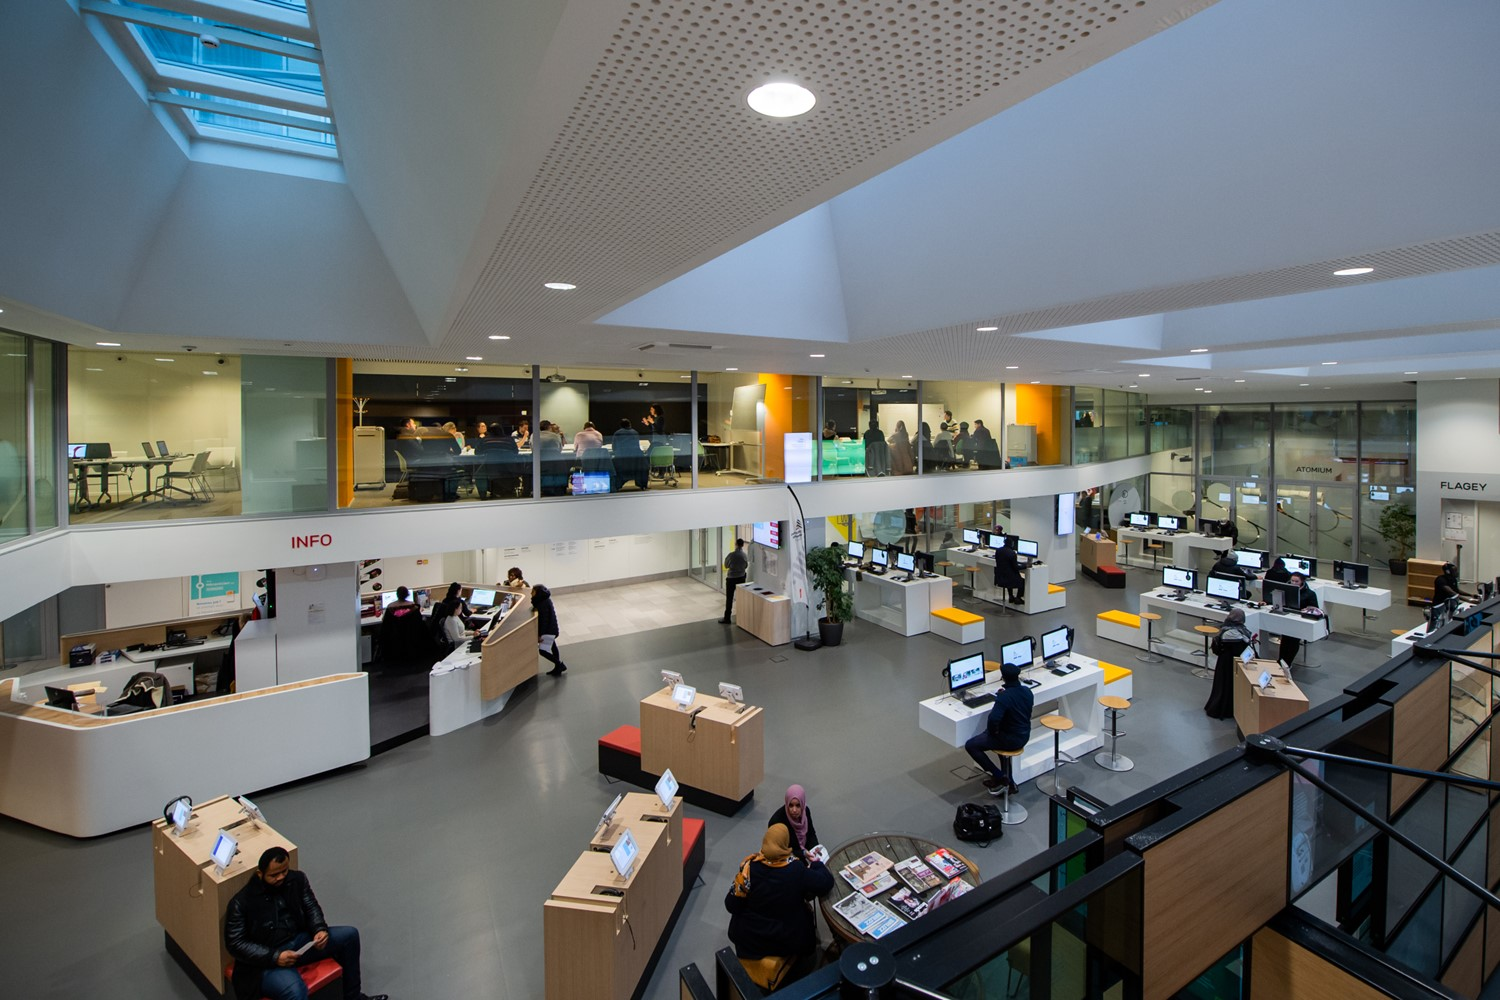
\includegraphics[scale=1]{imarina.JPG}~\\
\caption{Vue d'ensemble de la Cité des métiers de Bruxelles (Source: xxxx)}
\end{center}
\end{figure}


\newpage
\subsection{Etude de Cas 2}


\newpage
\subsection{Etude de Cas 3}

\newpage
\section{Conclusion}






\newpage
\begin{center}
\listoffigures
\end{center}

\newpage

\begin{center}
\bibliography{bibliographie}
\bibliographystyle{unsrtnat} 
\end{center}

\end{document}
